\chapter{First Approach: Single User MISO}

\section{Problem Realization}

\subsection{Channel Model}
We assume, there is 1 BS desires to send the data symbol $d$ to single user. The base stations employ $n_t$ transmit antennas and the user is equipped with a single receive antenna. BS employs a linear pre-coding column vector W of size $(n_t \times 1)$ prior to transmission over the air, which transforms the data symbol $d$ to the $(n_t \times 1)$ transmitted vector $\mathbf{X}=\mathbf{W}\ \cdot d$.
The channel from the BS to the user is represented by an $(1 \times n_t)$ row channel vector $h$ where \[ h = [h_1, h_2, \ldots, h_{n_t}] \] and $h_i$ denotes the path gain from the $i^{th}$ antenna of the BS to the user.

The channel elements are independently and identically distributed (i.i.d) according to $\mathcal{N}\mathcal{C}(0,1)$ i.e.,
$h \in {\mathbb{C}}^{1 \times n_t}$, the channel elements come from Rayleigh-fading distribution. \\
The received signal y at the user can be expressed as
\begin{equation}
    \label{eq:channel model}
    \begin{aligned}
        y &= h \cdot \mathbf{X} + n \\
        &= h \cdot \mathbf{W} \cdot d + n
    \end{aligned}
\end{equation}
where $n$ denotes complex-valued additive white Gaussian noise (AWGN) at user, distributed as $\mathcal{N}\mathcal{C}(0,\sigma^2_n)$

We impose the power constraint $\mathbb{E} \left\{ \text{tr}\left( \mathbf{X} \mathbf{X}^H \right)\right\}=1$ under assumption of unit-norm weight vectors $W$ and unit-power symbols $d_i$ i.e., $\|w\| = 1$.
And $\mathbb{E}\left\{ |d| \right\} = \sigma^2 d = 1$.
\begin{itemize}
    \item $\mathbb{E}[\cdot]$ denotes the expectation with respect to the distribution of the underlying random variable.
    \item $\text{tr}[\cdot]$ denotes the trace operator of a matrix.
    \item $\|\cdot\|$ indicates the 2-norm of a vector.
    \item $|\cdot|$ denotes the absolute value of a scalar.
\end{itemize}
Then the average transmits signal-to-noise ratio (SNR) of the network is defined as $\rho = \frac{1}{\sigma^2_n}$.

\subsection{Rate Equation}
Since our objective is to maximize the rate of each user so we now introduce Shannon rate equation:
\begin{equation}
    \label{eq:shannon rate}
    R = \log_2 \left( 1 + \frac{| h^H w |}{ \sigma^2_n } \right)
\end{equation}
Where our goal to find the best pre-coding vector $w$ which \textbf{maximizes the overall rate}.

\subsection{Optimization Formulation}
As we have mentioned our goal to maximize the rate (Equation~\ref{eq:shannon rate}) so now we formulate our problem as an usual optimization problem:
\begin{equation}
    \label{eq:rate opt}
    \begin{aligned}
        \max_w \qquad & \log_2 \left( 1 + \frac{| h^H w |}{ \sigma^2_n } \right) \\
        \text{s.t.} \qquad & \|w\|_2 = 1 \\
        & h, w \in \mathbb{C}^{n_t}
    \end{aligned}
\end{equation}
since we have constraint on pre-coding vector where the 2-norm square of pre-coding vector is equal to one which satisfies max power constraint since
\[ p_t = \|w\|^2_2 \cdot \sigma^2_d \]
And we have assumed that $\sigma^2_d = 1$ therefore $p_t$ tends to 1 (max power).

\section{RL Interpretation}
\subsection{Introduction}
After we have introduced the problem and formulated it as an optimization problem (Problem~\ref{eq:rate opt}) it is now time
to map it to an RL format but first we will answer the question of why we have started with the single user in the first place.\\
Since the SU problem has an analytical optimal solution when \[ w=\frac{h}{\|h\|} \] and it will help as to evaluate the problem and learn some tricks we will use in MU standard problem, so we have started with it as a confirmation of our approach.

\subsection{Problem Mapping}
As we have introduced in the previous chapter, to use RL algorithms we need to know its vocabulary state, action, and reward. Therefore, now we will apply the necessary mapping:
\begin{itemize}
    \item Channel $h_t$ to state $s_t$.
    \item Pre-coder vector $w_t$ to action $a_t$.
    \item Rate $R_t$ to reward $r_t$.
\end{itemize}
where: $\quad a_t, s_t \in \mathbb{C}^{n_t} \quad , \quad r_t \in \mathbb{R}$

\subsection{Algorithm Parameters}
\begin{enumerate}
    \item 3 hidden layer model with neurons [512,512,128] respectively.
    \item Actor learning rate = 0.001 and Critic learning rate = 0.002, we observe that critic learning rate bigger than actor learning rate because we need critic to guide the process of learning.
    \item Channel noise = 0.2.
    \item Exploration noise variance = 0.1 with decaying factor = 0.993.
    \item $\alpha, \beta, \gamma \in [0,1]$
\end{enumerate}

\subsection{Evaluation}
we evaluate the learned policies in terms of average rate using a test set of 5000 unseen samples. DDPG with PAE achieves more than 99\% of the maximum achievable rate.

\subsection{Optimization}
\subsubsection{Reward Shape}
\begin{wrapfigure}{H}{0.5\textwidth}
    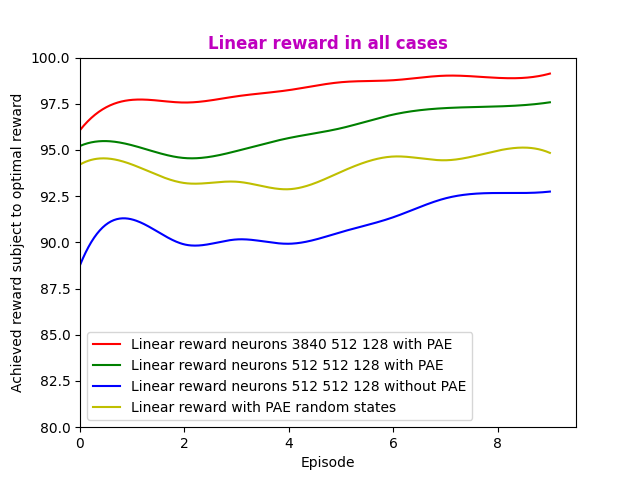
\includegraphics[width=0.5\textwidth]{H1.PNG}
    \caption{Achievable linear reward}
    \label{fig:linear reward}
\end{wrapfigure}
As we mentioned before, the reward the core of RL and it can direct the learning at any direction and as an example if I want to increase a robot speed to get out of the maze, we can make our reward a small negative reward to nudge the robot to complete fast to avoid punishment (refer to negative reward) so we have tried 2 versions of reward:\\\\
\textbf{1. Linear Reward} \\
We tried it first because it is faster and less computationally expensive, but it has a low performance compared to log reward and we observe that linear is still increasing which means it can reach to log reward but in more time.\\

\begin{wrapfigure}{H}{0.5\textwidth}
    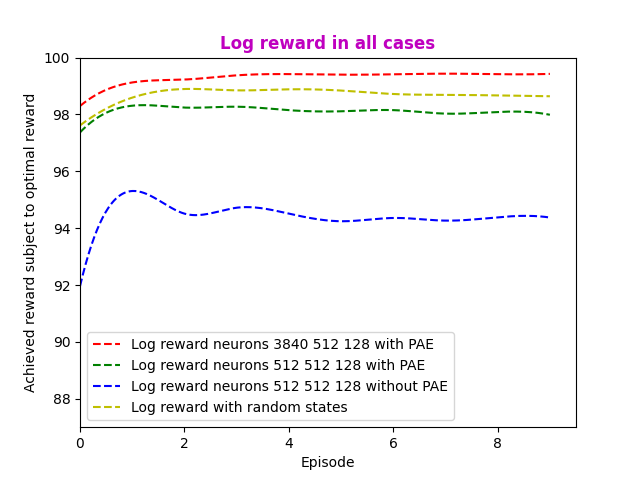
\includegraphics[width=0.5\textwidth]{H2.PNG}
    \caption{Achievable log reward}
    \label{fig:log reward}
\end{wrapfigure}
\textbf{2. Log Reward} \\
We tried it after bad performance of linear reward, and it gives better results but takes more time and computational power. \\

Observe the results of the comparison between linear and log rewards in Figure~\ref{fig:log and linear}. We observe that at constant environment log rate is higher than linear rate and faster. \\
The max percentage in case of \emph{linear}: \textbf{99.134\%} at \textbf{episode = 9}.\\
The max percentage in case of \emph{log}: \textbf{99.435\%} at \textbf{episode = 7}.

\begin{figure}[ht]
    \centering
    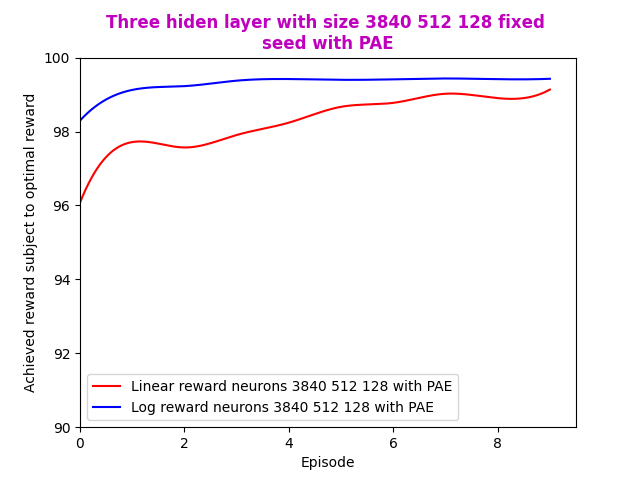
\includegraphics[width=0.7\textwidth]{H3.png}
    \caption{Linear \& log rewarding techniques comparison}
    \label{fig:log and linear}
\end{figure}

\subsubsection{Phase Ambiguity Elimination}
We address the phase ambiguity issue in the commonly used vector (or matrix) representation of wireless channel states and then present a method to improve DDPG training in MISO.\\
In radio communications, a pass-band channel state is represented by a complex-valued base-band equivalent. In our signal model, the channel vectors $h$ can be expressed as a complex-valued representation with respect to amplitude and phase, denoted by
\begin{equation}
    c = \left[ a_1 \exp\left( \jmath \vartheta_1 \right), a_2 \exp\left( \jmath \vartheta_2 \right), \ldots, a_{n_t} \exp\left( \jmath \vartheta_{n_t} \right) \right]
\end{equation}
where $a_i$ and $\vartheta_i$ are the amplitude and phase of the $i^{th}$ element of vector $c$ respectively. \\
We note that the channel state given by $c$ has inherent phase ambiguity resulting from the complex-valued base-band signal representation.
More specifically, all the phase-shifted states $\exp\left( \jmath \phi \right)$ c with arbitrary phases $\phi$ are supposed to lead to the same action as that of the original state $c$. \\

From the wireless system design point of view, this phase ambiguity should not be a problem, but it introduces a \emph{(many-to-one mapping)} issue between a set of phase-shifted states with different offsets and one target optimal action, which further complicates the
training task, and thereby, degrades the performance in a multi agent learning system. To combat the degradation due to the many-to-one mapping nature of state-action pairs,
we propose a \emph{PAE} method as a pre-processing on channel states $h$, that maps channel states with phase ambiguity into the same state. The training method can be utilized. \\

Any mapping function $f_{\text{PAE}}(\cdot)$ that eliminates inherent phase ambiguity. For instance, we consider a PAE mapping function that maps each state $c$ onto one state whose first element is purely real valued as follows:
\begin{equation}
    \label{Mapping function}
    f_{\text{PAE}}(c) = \left[ a_1 , a_2 \exp \left( \jmath \left( \vartheta_2 - \vartheta_1 \right) \right) , \ldots , a_{n_t} \exp \left( \jmath \left( \vartheta_{n_t} - \vartheta_1 \right) \right) \right]
\end{equation}
\textbf{In summary,} the final state representation can be obtained by applying the mapping function $f_{\text{PAE}}$ to $h$ as $s^{\text{PAE}} = \left[ f_{\text{PAE}}(h) \right]$ \\
\begin{wrapfigure}{ht}{0.5\textwidth}
    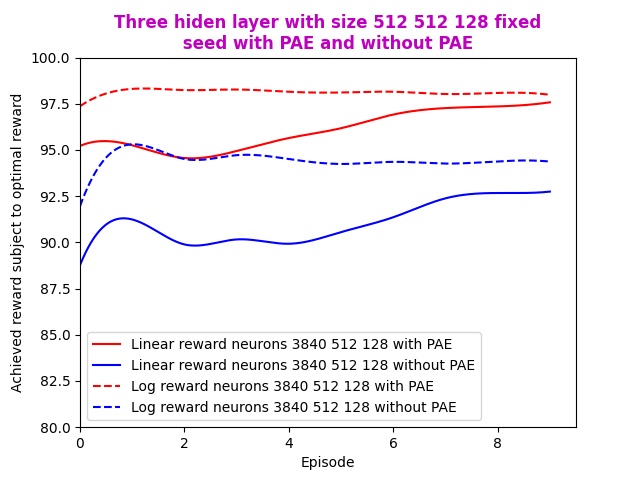
\includegraphics[width=0.5\textwidth]{H4.PNG}
    \caption{Achievable rewards with and without PAE}
    \label{fig:Achievable rewards with and without PAE}
\end{wrapfigure}

Figure~\ref{fig:Achievable rewards with and without PAE} depicts the achievable reward subject to the optimal reward for both techniques with and without PAE. It shows that the proposed PAE training method can achieve a faster convergence and a better performance compared to the trivial approach given without consideration of phase ambiguity elimination.
\begin{itemize}
    \item The max percentage in case of \textbf{linear with PAE}: 97.58\%.
    \item The max percentage in case of \textbf{linear without PAE}: 92.75\%.
    \item The max percentage in case of \textbf{log with PAE}: 98.3\%.
    \item The max percentage in case of \textbf{log without PAE}: 95.3\%. 
\end{itemize}

\subsubsection{Changing Seed}
We make the seed fixed because it make the process faster due to taking same trajectory every time. \\
\begin{wrapfigure}[8]{ht}{0.5\textwidth}
    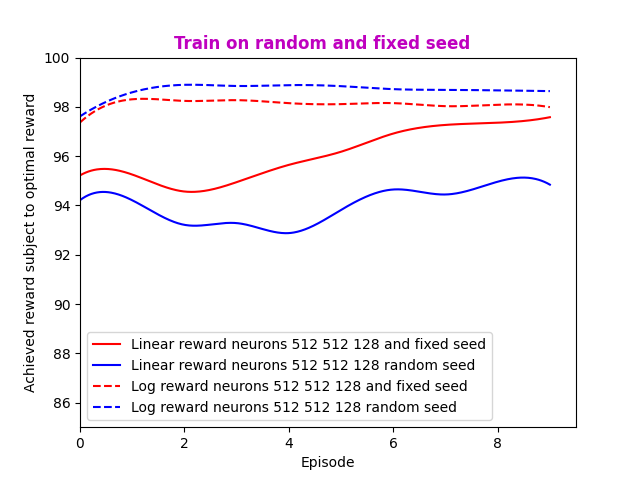
\includegraphics[width=0.5\textwidth]{H5.PNG}
    \caption{Training on random and fixed seeds}
    \label{fig:random and fixed}
\end{wrapfigure}
Figure~\ref{fig:random and fixed} depicts the achievable reward subject to the optimal reward for both techniques with fixed and random seeds.
\begin{itemize}
    \item The max percentage in case of \textbf{linear with fixed seed}: 97.58\%.
    \item The max percentage in case of \textbf{linear with random seed}: 94.96\%.
    \item The max percentage in case of \textbf{log with fixed seed}: 98.31\%.
    \item The max percentage in case of \textbf{log with random seed}: 98.89\%. 
\end{itemize}

\subsection{Challenges}
\subsubsection{NNs Inputs}
It is known that neural networks can not process complex numbers of channel which comes from the nature of the problem, so we have solved it by making some manipulation to force the inputs to be consistent with NNs so, we have created a function which split complex number to real and imaginary so $s_t=\left\{\text{real}\left(h_t\right),\text{img}(h_t)\right\}$ and same thing to $a_t$ then we found that $a_t, s_t \in \mathbb{R}^{2n_t}$. \\
So $w_t=a_t\left[1:n_t\right]+\jmath a_t[n_t+1:2n_t]$
\begin{figure}[ht]
    \centering
    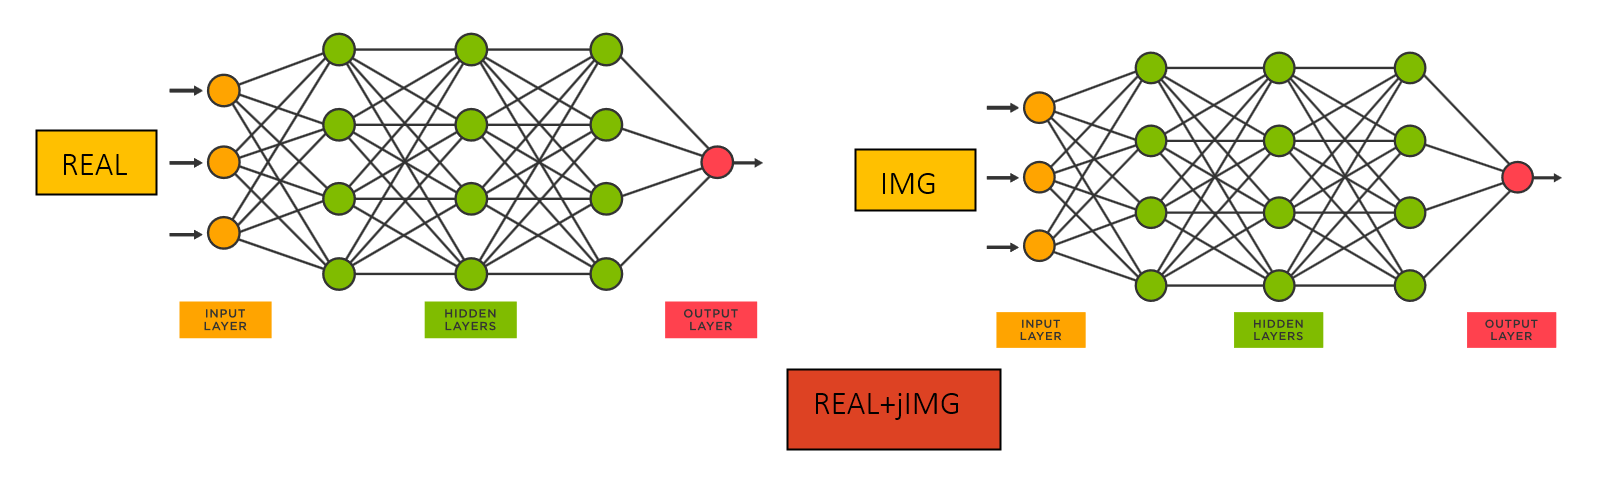
\includegraphics[width=0.8\textwidth]{H6.png}
    \caption{Real and imaginary NNs}
    \label{fig:real and img}
\end{figure}

\subsubsection{Custom Layer}
First, we had a problem with achieving power constraint where we needed 2-norm of $w_t$ To be equal 1 which need normalization along all $w_t$ from all antennas. \\
To achieve this goal, \emph{we tried 2 methods}:
\begin{enumerate}
    \item we tried to normalize the final action (pre-coder)output of “relu” function of the actor with normal normalization which caused problems due to non-learnable parameters of the function.
    \item designed custom normalization layer which can learn and update each parameter to add error sense to critic.
\end{enumerate}

\subsubsection{Hyper-parameter Tunning}

\begin{wrapfigure}[10]{r}{0.5\textwidth}
    \vspace{-25pt}
    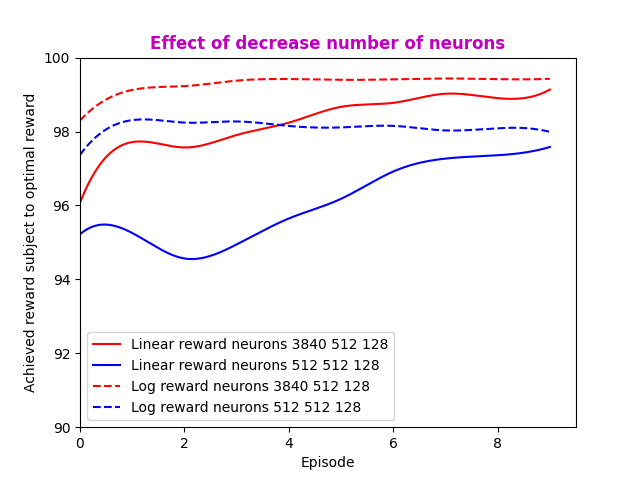
\includegraphics[width=0.5\textwidth]{H7.PNG}
    \caption{Effect of decreasing neurons}
    \label{fig:decreasing neurons}
\end{wrapfigure}
To further improve the performance of the algorithm, we tried the following:
\begin{itemize}
    \item Learning rate tunning (to achieve better convergence).
    \item Defining a discounting factor.
    \item Decreasing number of layers' neurons (as shown in Figure~\ref{fig:decreasing neurons}).
\end{itemize}
This achieved lower performance in same running time for both linear and log reward, but gets better and better as it runs for more episodes.
\begin{itemize}
    \item The max percentage in case of \textbf{linear for big model}: 99.14\%.
    \item The max percentage in case of \textbf{linear}: 97.58\%.
    \item The max percentage in case of \textbf{log for big model}: 99.44\%.
    \item The max percentage in case of \textbf{log}: 98.31\%.
\end{itemize}

\subsubsection{General Comparasion}
Figure~\ref{fig:all} depicts the comparison between all the versions of the algorithm based on its achievable reward subject to the optimal reward.
\begin{figure}[ht]
    \centering
    \vspace{-10pt}
    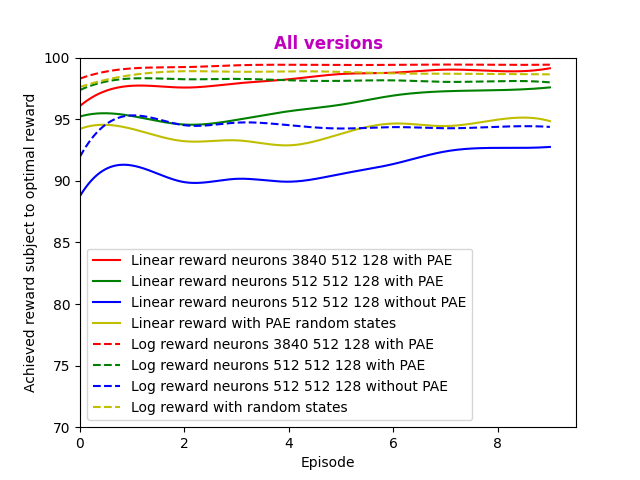
\includegraphics[width=0.7\textwidth]{H8.png}
    \caption{All versions of the model}
    \label{fig:all}
\end{figure}

\subsection{Pseudo Code}
\vspace{-30pt}
\begin{samepage}
\begin{algorithm}
    \caption{Algorithm of finding the optimal pre-coding vector for Single User MISO}
    \label{alg:single-user}
    \begin{algorithmic}
        \State Initialize actor network $\text{actor}_{\theta^a}(s)$ and critic network $\text{critic}_{\theta^Q}(s,a)$ with random parameters $\phi$ and $\vartheta$ using Xavier.
        \State $\sigma^2_\epsilon \gets 0.1$
        \For{episode $i = 1, n_\text{episode}$}
            \State Initialize the initial state $s_0$ of sequence according to the channel model.
            \For{time step $j = 0 , n_\text{time steps}$}
                \State Choose an action $a_t = \text{actor}_\phi(s_t = h_t) + \acute{\mathbf{N}}$ with exploration noise $\acute{\mathbf{N}} \in \mathcal{N} \mathcal{C}  \left( 0, \sigma^2_\epsilon \right)$.
                \State Execute action $a_t$ in environment to get reward \[ r_t = \log_2 \left( 1 + \frac{ |h^Hw| }{\sigma^2_n} \right) \]
                \State Observe the next state $s_{t+1} = h_{t+1}$.
                \State Buffer $(s_t, a_t, r_t, s_{t+1})$ to memory.
                \State Compute the loss function \Comment{Start of the learning process}
                \begin{equation}
                    \begin{aligned}
                        y_t &= r_i + \gamma \cdot \text{target critic}_{\theta^{Q'}} \left( s_{t+1} , \text{target actor}_{\theta^{a'}}(s_{t+1}) \right) \\
                        \mathbf{L} &= \frac{1}{M} \sum_{t} \left( y_t - \text{critic}_{\theta^Q}(s_t, a_t) \right)^2 \\
                        \text{w.r.t.} & \text{ target value } \mathbf{Y}^{\theta^Q}_t \text{ and } \text{critic}_{\theta^Q}(s_t, a_t)
                    \end{aligned}
                \end{equation}
                \State Compute the gradient vector $\nabla_{\theta^Q} \mathbf{L}(\theta^Q)$ on the experience $(s_t, a_t, r_t, s_{t+1})$.
                \State Update the critic network as \[ \theta^Q \gets \theta^Q - \beta \nabla_{\theta^Q} \mathbf{L}(\theta^Q) \]
                \State Compute the gradient vector \[ \nabla_{\theta^a} \mathbf{J}(\theta^a) = \left( \nabla_{\theta^a} \text{actor}(\theta^a) |_{s=s_t} \right) \left( \nabla_{a} \text{critic}(s,a)|_{s=s_t , a = \text{actor}(s_t)} \right) \]
                \State Update the actor network as \[ \theta_a \gets \theta_a + \alpha \nabla_{\theta^a} \mathbf{J}(\theta_a) \]
                \State Soft Update
                \begin{equation}
                    \begin{aligned}
                        \theta_{Q'} & \gets \tau \theta_Q + (1 - \tau) \theta_{Q'} \\
                        \theta_{a'} & \gets \tau \theta_a + (1 - \tau) \theta_{a'} \\
                    \end{aligned}
                \end{equation} 
                \State Evaluate over 5000 unseen states. \Comment{End of learning process}
            \EndFor
            \State $\sigma^2_\epsilon \gets \sigma^2_\epsilon \times 0.993$
        \EndFor
    \end{algorithmic}
\end{algorithm}
\end{samepage}